
\documentclass[11pt]{article}

\usepackage{indentfirst}
\usepackage{url}

\RequirePackage{amsmath}
\newcommand{\boldbeta}{{\boldsymbol{\beta}}}
\newcommand{\boldeta}{{\boldsymbol{\eta}}}
\newcommand{\boldtheta}{{\boldsymbol{\theta}}}
\newcommand{\boldthetahat}{{\boldsymbol{\hat{\theta}}}}
\newcommand{\boldxi}{{\boldsymbol{\xi}}}
\newcommand{\boldtau}{{\boldsymbol{\tau}}}
\newcommand{\boldvarphi}{{\boldsymbol{\varphi}}}
\newcommand{\boldzeta}{{\boldsymbol{\zeta}}}
\newcommand{\boldA}{{\mathbf{A}}}
\newcommand{\boldB}{{\mathbf{B}}}
\newcommand{\boldM}{{\mathbf{M}}}

% \VignetteIndexEntry{Aster Package Tutorial}

\usepackage{/usr/local/lib/R/share/texmf/Sweave}
\begin{document}

\title{The Aster Package Tutorial}
\author{Charles J. Geyer}
\maketitle


\section{Preliminaries}

\subsection{Warning} \label{sec:warn}

A redesign of the calling sequence of the functions
\begin{verbatim}
aster
predict.aster
predict.aster.formula
\end{verbatim}
is underway.  Some of the details of what follows is likely
to change in a future version (real soon now).

\subsection{Library and Data}

\begin{Schunk}
\begin{Sinput}
> library(aster)
> data(echinacea)
\end{Sinput}
\end{Schunk}
That's our package and the dataset for our examples.

\subsection{Digression on Data Entry}

The simplest way to enter your own data into R is to construct a plain
text file that is a white-space-separated matrix of
numbers with column headings.
(Note this means not touched by Microsoft Word or any so-called
word processors that are incapable of not garbaging up plain text
with a lot of unwanted formatting junk: if on Microsoft Windows,
use Microsoft Notepad.)

An example is the file
\verb@"echinacea.txt"@ found in the \verb@data@ directory of the
package installation.

This file could read into R as follows
\begin{verbatim}
echinacea <- read.table("echinacea.txt", header = TRUE)
\end{verbatim}
In fact that's what R did when loading the library.

If you have been so foolish as to give your data to Microsoft Excel,
you can ask it to give it back by writing out in CSV (Microsoft
comma separated values format), and it may give you back something usable
(or it may not: dates are expecially problematic, for some reason).
If the output is called \verb@echinacea.csv@ then
\begin{verbatim}
echinacea <- read.csv("echinacea.csv")
\end{verbatim}
will read it into R.

\subsection{Digression on Data Frames}

In either case the R object \verb@echinacea@ created by the \verb@data@
statement or a \verb@read.table@
or \verb@read.csv@ command is what R calls a \emph{data frame}.  It prints like
a matrix but is really a list of vectors of the same length.  The command
\begin{Schunk}
\begin{Sinput}
> names(echinacea)
\end{Sinput}
\begin{Soutput}
 [1] "hdct02" "hdct03" "hdct04" "site"   "ewloc"  "nsloc" 
 [7] "ld02"   "fl02"   "ld03"   "fl03"   "ld04"   "fl04"  
\end{Soutput}
\end{Schunk}
shows the names of these (vector) variables.  The names are the column
headings from the input file.  Any variables having character values
have been coerced to what R calls \emph{factors}.  To see what kind of
variable each is we can do
\begin{Schunk}
\begin{Sinput}
> sapply(echinacea, class)
\end{Sinput}
\begin{Soutput}
   hdct02    hdct03    hdct04      site     ewloc     nsloc 
"integer" "integer" "integer"  "factor" "integer" "integer" 
     ld02      fl02      ld03      fl03      ld04      fl04 
"integer" "integer" "integer" "integer" "integer" "integer" 
\end{Soutput}
\end{Schunk}

In the \verb@echinacea@ data set,
the variables with numbers in the names are the columns of the response
matrix of the aster model.
\begin{itemize}
\item
The variables \verb@ld0@$x$ (where $x$ is
a digit) are the survival indicator variables for year 200$x$
(one for alive, zero for dead).
\item
The variables \verb@fl0@$x$ are the flowering indicator variables
(one for any flowers, zero for none).
\item
The variables \verb@hdct0@$x$ are the inflorescence (flower head) count
variables (number of flower heads).
\end{itemize}
The variables without numbers are other predictors.
\begin{itemize}
\item
The variables \verb@ewloc@ and \verb@nsloc@ are spatial, east-west
and north-south location, respectively.  
\item
The variable \verb@site@ is the site of origin of the plant, so plants
with different values of \verb@site@ may be more genetically diverse
than those with the same values of \verb@site@.
\end{itemize}

The point of recording the data about flowers in two variables
\verb@fl0@$x$ and \verb@hdct0@$x$ for any given $x$ when the
single variable \verb@hdct0@$x$ contains the same information
(because \verb@fl0@$x$ = 0 if and only if \verb@hdct0@$x$ = 0)
is because there is no good, simple statistical model for \verb@hdct0@$x$
by itself.

As we shall see, it makes sense to model the conditional distribution of
\verb@fl0@$x$ given \verb@ld0@$x$ = 1 as Bernoulli and it makes sense
to model the conditional distribution of
\verb@hdct0@$x$ given \verb@fl0@$x$ = 1 as Poisson conditioned on being
nonzero.  But it would not make sense to model \verb@hdct0@$x$
given \verb@ld0@$x$ = 1 as Poisson.  The case of zero flowers is special
and must be modeled separately.

\subsection{Digression on Reshape}

Standard regression-like modeling requires that the ``response'' be
a vector.  The ``response'' (``data'' would be a better name since it
plays two roles: $X_{i p(j)}$ is the sample size for $X_{i j}$) is a
matrix.  If we are going to use any of the R apparatus for doing
regression-like modeling, in particular if we are going to use the
R formula mini-language that allows model specifications like
\verb@y ~ x1 + x2@ then we need to make the response (the \verb@y@
in the formula) a vector.

There is an R function \verb@reshape@ that does this
\begin{Schunk}
\begin{Sinput}
> vars <- c("ld02", "ld03", "ld04", "fl02", "fl03", 
+     "fl04", "hdct02", "hdct03", "hdct04")
> redata <- reshape(echinacea, varying = list(vars), 
+     direction = "long", timevar = "varb", times = as.factor(vars), 
+     v.names = "resp")
> names(redata)
\end{Sinput}
\begin{Soutput}
[1] "site"  "ewloc" "nsloc" "varb"  "resp"  "id"   
\end{Soutput}
\end{Schunk}
making a new data frame (in this case \verb@redata@) that has new
variables (all of the same length because they are in the same data frame)
\begin{description}
\item[\normalfont \texttt{resp}] which contains all of the data in the
variables indicated by the string \verb@vars@ packed into a single vector, the
name \verb@resp@ being given by the \verb@v.names@ argument of the
\verb@reshape@ function (you could make it anything you like),
\item[\normalfont \texttt{varb}] which indicates which original variable the
corresponding
element of \verb@resp@ came from, the name being given by the \verb@timevar@
argument of the \verb@reshape@ function, and
\item[\normalfont \texttt{id}] which indicates which original individual the
corresponding
element of \verb@resp@ came from, the name being given by the \verb@idvar@
argument of the \verb@reshape@ function (which we didn't specify, accepting
the default value \verb@"id"@).
\end{description}

\paragraph{Warning} The variable \verb@vars@ must have the variables
listed with parent nodes before child nodes.  This doesn't make sense
now, but is nessary to satisfy condition \eqref{eq:foo}
on page~\pageref{eq:foo}.

\medskip
Let's look at an example
\begin{Schunk}
\begin{Sinput}
> redata[42, ]
\end{Sinput}
\begin{Soutput}
        site ewloc nsloc varb resp id
42.ld02  SPP    -3     7 ld02    1 42
\end{Soutput}
\end{Schunk}
This says that the 42nd row of the data frame \verb@redata@ has response
value 1.  This is the response for the
\texttt{ld02} original variable
(node of the graphical model)
and for individual 42 found
in row 42
of the original data frame \verb@echinacea@.  The other variables \verb@site@,
\verb@ewloc@, and \verb@nsloc@ are what they were in this row
of \verb@echinacea@
(for this original individual) and are duplicated as necessary in other
rows of \verb@redata@.

\section{Unconditional Aster Models}

Now we are ready to begin discussion of Aster models.
First we load the package.
\begin{Schunk}
\begin{Sinput}
> library(aster)
\end{Sinput}
\end{Schunk}

\subsection{More Preliminaries}

Then more details.  We must define a few more variables that determine
the structure of the aster model we intend to work with.  The variable
\verb@resp@ contains only the random data.  There is also the non-random
data on the root nodes of the dependence graph of the model.  For reasons
having to do with the way the R formula mini-language works, we usually
want this in the same data frame as \verb@resp@
\begin{Schunk}
\begin{Sinput}
> redata <- data.frame(redata, root = 1)
> names(redata)
\end{Sinput}
\begin{Soutput}
[1] "site"  "ewloc" "nsloc" "varb"  "resp"  "id"    "root" 
\end{Soutput}
\end{Schunk}
This adds a variable \verb@root@ to the data frame and makes all its values
one (including for non-root nodes, but those values are ignored by
all \verb@aster@ package functions).

We also need two vectors of the same length as the number of nodes in the
graph (so they cannot go in the data frame \verb@redata@),
call that length \verb@nnode@
\begin{Schunk}
\begin{Sinput}
> pred <- c(0, 1, 2, 1, 2, 3, 4, 5, 6)
> fam <- c(1, 1, 1, 1, 1, 1, 3, 3, 3)
> families()[fam]
\end{Sinput}
\begin{Soutput}
[1] "bernoulli"        "bernoulli"        "bernoulli"       
[4] "bernoulli"        "bernoulli"        "bernoulli"       
[7] "non.zero.poisson" "non.zero.poisson" "non.zero.poisson"
\end{Soutput}
\end{Schunk}
\begin{description}
\item[\normalfont \texttt{pred}] specifies the predecessor structure of
the graph.  With the original variables indexed from 1 to \verb@nnode@,
in the order that they appear in the variable \verb@vars@ defined above
and supplied as the \verb@varying@ argument to the \verb@reshape@ function,
\verb@pred[j]@ gives the index of the predecessor of node \verb@j@.
In order to make it obvious that \verb@pred@ specifies an acyclic graph,
we require
\begin{equation} \label{eq:foo} \tag{$*$}
\verb@all(pred < seq(along = pred))@
\end{equation}
hold.  If \verb@pred[j] == 0@ this indicates \verb@j@ indexes a root node
(no predecessor).
\item[\normalfont \texttt{fam}] specifies the one-parameter exponential
families for the nodes: \verb@fam[j]@ gives the index of the family for
node \verb@j@, the index being for the vector of family names returned
by \verb@families()@.
\end{description}

\paragraph{Comment}  Using an index vector rather than a character vector
for \verb@fam@ is definitely not the R way.  But having decided
to make \verb@pred@ an index vector, the same seemed natural for \verb@fam@.

The reason for using an index vector for \verb@pred@ is so the condition
\eqref{eq:foo} makes sense.  The original variables must be related to
their order in the data frame \verb@redata@ in any case.

\paragraph{Warning}
This may change in the future, but that's the way it is for now.
In fact it is very likely to change in the future and in a
non-backwards-compatible way (see the warning in Sec~\ref{sec:warn}).

\subsection{Fitting a Model}

We are finally ready to fit a model.
\begin{Schunk}
\begin{Sinput}
> aout1 <- aster(resp ~ varb + nsloc + ewloc + site, 
+     pred, fam, varb, id, root, data = redata)
> summary(aout1, show.graph = TRUE)
\end{Sinput}
\begin{Soutput}
Call:
aster.formula(formula = resp ~ varb + nsloc + ewloc + site, pred = pred, 
    fam = fam, varvar = varb, idvar = id, root = root, data = redata)


Graphical Model:
 variable predecessor family          
 ld02     root        bernoulli       
 ld03     ld02        bernoulli       
 ld04     ld03        bernoulli       
 fl02     ld02        bernoulli       
 fl03     ld03        bernoulli       
 fl04     ld04        bernoulli       
 hdct02   fl02        non.zero.poisson
 hdct03   fl03        non.zero.poisson
 hdct04   fl04        non.zero.poisson

             Estimate Std. Error z value Pr(>|z|)    
(Intercept) -1.429438   0.184006  -7.768 7.95e-15 ***
varbfl03    -0.329497   0.265611  -1.241  0.21478    
varbfl04    -0.355326   0.241242  -1.473  0.14078    
varbhdct02   1.715376   0.249520   6.875 6.21e-12 ***
varbhdct03   1.733264   0.200166   8.659  < 2e-16 ***
varbhdct04   2.246177   0.185538  12.106  < 2e-16 ***
varbld02    -0.967928   0.311876  -3.104  0.00191 ** 
varbld03     0.793777   0.392935   2.020  0.04337 *  
varbld04     3.932665   0.330810  11.888  < 2e-16 ***
nsloc        0.013684   0.001733   7.895 2.91e-15 ***
ewloc        0.006003   0.001727   3.475  0.00051 ***
siteEriley  -0.052273   0.053504  -0.977  0.32857    
siteLf      -0.046125   0.056892  -0.811  0.41751    
siteNWLF    -0.061712   0.051028  -1.209  0.22652    
siteNessman -0.124857   0.070894  -1.761  0.07821 .  
siteSPP      0.036007   0.054506   0.661  0.50887    
siteStevens -0.084581   0.054256  -1.559  0.11901    
---
Signif. codes:  0 `***' 0.001 `**' 0.01 `*' 0.05 `.' 0.1 ` ' 1 
\end{Soutput}
\end{Schunk}
The \verb@show.graph = TRUE@ makes the table about the graph structure
in the printout.  You always want to look at that carefully once, since
it tells you whether you have gotten it right.  But (unless you change
\verb@redata@, \verb@pred@, or \verb@fam@) it won't change thereafter.
Hence the default is to not print it.

\paragraph{Interpretation.} From looking at the ``signif.\ stars''
it looks like \verb@site@ is not significant.  But you're not supposed
to use ``signif.\ stars'' that way.  Any use of more than one
``signif.\ stars'' per model fit is \emph{multiple testing without correction}
and may be \emph{highly misleading}.  Wise users put
\begin{Schunk}
\begin{Sinput}
> options(show.signif.stars = FALSE)
\end{Sinput}
\end{Schunk}
in their \verb@.Rprofile@ file so they aren't even tempted to foolishness
by them.  The R default is to print them, so that's what \verb@summary.aster@
does too.

\subsection{Model Comparison}

The right way to compare models is with a likelihood ratio test.
To do that, you must fit two models.  So here's another.
\begin{Schunk}
\begin{Sinput}
> aout2 <- aster(resp ~ varb + nsloc + ewloc, pred, 
+     fam, varb, id, root, data = redata)
\end{Sinput}
\end{Schunk}
Now we can compare them with
\begin{Schunk}
\begin{Sinput}
> anova(aout2, aout1)
\end{Sinput}
\begin{Soutput}
Analysis of Deviance Table

Model 1: resp ~ varb + nsloc + ewloc
Model 2: resp ~ varb + nsloc + ewloc + site
  Model Df Model Dev Df Deviance P(>|Chi|)
1       11   2747.90                      
2       17   2734.38  6    13.52      0.04
\end{Soutput}
\end{Schunk}

So much for making inferences from a bunch of signif.\ stars!
Not one of the signif.\ stars for the \verb@site@ dummy variables
in the printout for \verb@aout1@ was anywhere near as significant
as the likelihood ratio test $p$-value here.  See what we mean?

\paragraph{Warning} (copied from the \verb@anova.aster@ help page)
\begin{quote}
     The comparison between two or more models \ldots
     will only be valid if they are (1) fitted to the
     same dataset, (2) models are nested, (3) models are of the same
     type (all conditional or all unconditional), (4) have the same
     dependence graph and exponential families. None of this is
     currently checked.
\end{quote}
You're not likely to botch (1) or (4).  Just make sure you use the
same data frame and the same \verb@pred@ and \verb@fam@.  If you're
a little careful, you won't botch (3).  We haven't done conditional
models yet (see Section~\ref{sec:conditional}), but if careful one
should not botch that (conditional and unconditional models are like
apples and oranges, they shouldn't be mixed).  The hard condition
to always obey is (2).  One must be sure that the column space of
the model matrix of the big model (\verb@aout1$modmat@) contains
the column space of the model matrix of the small model (\verb@aout2$modmat@),
but that is much easier checked by the computer than by you.

\paragraph{Comment} So perhaps the computer should check all this,
despite none of the R \verb@anova@ functions doing so.  It would take
time, enough for one linear regression per column of the model matrix
of the small model.  But it would add safety.  But the R/C/Unix way
(a.~k.~a., worse is better) is to not check and let the user worry
about it.

Anyway (as the warning says) \verb@anova.aster@ and \verb@anova.asterlist@
currently do not check.  The user must make sure the models are nested
(otherwise the comparison is theoretically rubbish).

\subsection{Models Based on Pseudo-Covariates}

In a sense the ``covariate'' variable \verb@varb@ is already a
pseudo-covariate.  It's not a measured variable.  It's an artifice
we use to overcome the limitations of the R formula mini-language
insisting that the ``response'' be a vector, rather than a matrix
with heterogenous columns (like it really is).

In this section we do more artifice.  The variables of interest,
that are ``components of fitness'' in the evolutionary jargon
are the \verb@hdct@ variables.  We want to look that the interaction
of site with those variables.  So first we have to create the relevant
dummy variable.
\begin{Schunk}
\begin{Sinput}
> hdct <- grep("hdct", as.character(redata$varb))
> hdct <- is.element(seq(along = redata$varb), hdct)
> redata <- data.frame(redata, hdct = as.integer(hdct))
> names(redata)
\end{Sinput}
\begin{Soutput}
[1] "site"  "ewloc" "nsloc" "varb"  "resp"  "id"    "root" 
[8] "hdct" 
\end{Soutput}
\end{Schunk}
This is tricky.  The variable \verb@redata$varb@ is a factor,
which means it is really numeric (an index vector) under the hood,
even though it prints as a character string.  To get the
strings to work with we do \verb@as.character(redata$varb)@.
Then the first statement returns the \emph{indices} of the elements
of \verb@varb@ whose string forms contain \verb@"hdct"@.  The next
statement converts these to \verb@TRUE@ or \verb@FALSE@.
The third statement converts these to one and zero, and makes them
the variable \verb@hdct@ in the data frame \verb@redata@.
You might not think of such an R-ish way to do this, but if
you want to use such a variable in modeling, you must create it
somehow.

Now we can fit an interaction term.
\begin{Schunk}
\begin{Sinput}
> aout3 <- aster(resp ~ varb + nsloc + ewloc + site * 
+     hdct, pred, fam, varb, id, root, data = redata)
> summary(aout3)
\end{Sinput}
\begin{Soutput}
Call:
aster.formula(formula = resp ~ varb + nsloc + ewloc + site * 
    hdct, pred = pred, fam = fam, varvar = varb, idvar = id, 
    root = root, data = redata)

                  Estimate Std. Error z value Pr(>|z|)
(Intercept)      -1.583649   0.216993  -7.298 2.92e-13
varbfl03         -0.328716   0.264185  -1.244 0.213403
varbfl04         -0.339642   0.239818  -1.416 0.156702
varbhdct02        1.996726   0.323007   6.182 6.34e-10
varbhdct03        2.014335   0.287024   7.018 2.25e-12
varbhdct04        2.525820   0.277131   9.114  < 2e-16
varbld02         -0.971302   0.312215  -3.111 0.001865
varbld03          0.775863   0.393076   1.974 0.048402
varbld04          3.897397   0.330949  11.776  < 2e-16
nsloc             0.013538   0.001727   7.838 4.59e-15
ewloc             0.005990   0.001724   3.474 0.000513
siteEriley        0.332627   0.152129   2.186 0.028780
siteLf            0.318859   0.162391   1.964 0.049584
siteNWLF          0.017505   0.142818   0.123 0.902449
siteNessman       0.211191   0.187665   1.125 0.260435
siteSPP           0.168390   0.156462   1.076 0.281822
siteStevens      -0.083259   0.150749  -0.552 0.580741
siteEriley:hdct  -0.717275   0.259529  -2.764 0.005714
siteLf:hdct      -0.678378   0.278899  -2.432 0.015001
siteNWLF:hdct    -0.127151   0.241487  -0.527 0.598518
siteNessman:hdct -0.673876   0.354761  -1.900 0.057496
siteSPP:hdct     -0.238292   0.258664  -0.921 0.356924
siteStevens:hdct  0.027072   0.256538   0.106 0.915956

Original predictor variables dropped (aliased)
     hdct 
\end{Soutput}
\end{Schunk}

\paragraph{Comment}  The \verb@dropped (aliased)@ means just what
it says.  The R formula mini-language does not deal correctly with
pseudo-covariates like this and thinks it should put (a dummy variable
for) \verb@hdct@ in the model, but that is aliased with the sum of
(the dummy variables for) \verb@varbhdct02@, \verb@varbhdct03@,
and \verb@varbhdct04@, so the \verb@aster@ function drops it, but
not silently (so the user is not surprised).

It turns out this is not the model we wanted to fit.  We didn't want
site main effects, \verb@siteEriley@ and so forth, \emph{in addition to}
the site interaction effects \verb@siteEriley:hdct@ and so forth.  We
only wanted \verb@site@ to have effects at the \verb@hdct@ level.
Here's how we do that
\begin{Schunk}
\begin{Sinput}
> aout4 <- aster(resp ~ varb + nsloc + ewloc + site * 
+     hdct - site, pred, fam, varb, id, root, data = redata)
> summary(aout4)
\end{Sinput}
\begin{Soutput}
Call:
aster.formula(formula = resp ~ varb + nsloc + ewloc + site * 
    hdct - site, pred = pred, fam = fam, varvar = varb, idvar = id, 
    root = root, data = redata)

                  Estimate Std. Error z value Pr(>|z|)
(Intercept)      -1.463638   0.178183  -8.214  < 2e-16
varbfl03         -0.328488   0.265142  -1.239 0.215377
varbfl04         -0.349519   0.240775  -1.452 0.146601
varbhdct02        1.808447   0.258014   7.009 2.40e-12
varbhdct03        1.825590   0.210824   8.659  < 2e-16
varbhdct04        2.338955   0.197099  11.867  < 2e-16
varbld02         -0.989146   0.311742  -3.173 0.001509
varbld03          0.776572   0.392815   1.977 0.048049
varbld04          3.918323   0.330729  11.848  < 2e-16
nsloc             0.013600   0.001729   7.867 3.64e-15
ewloc             0.006473   0.001725   3.753 0.000174
siteEriley:hdct  -0.173902   0.089753  -1.938 0.052676
siteLf:hdct      -0.157706   0.096580  -1.633 0.102490
siteNWLF:hdct    -0.109268   0.083325  -1.311 0.189740
siteNessman:hdct -0.315681   0.139822  -2.258 0.023962
siteSPP:hdct      0.023541   0.086552   0.272 0.785630
siteStevens:hdct -0.127403   0.089518  -1.423 0.154677

Original predictor variables dropped (aliased)
     hdct 
\end{Soutput}
\end{Schunk}
and here's the ANOVA (analysis of deviance, log likelihood ratio test)
table for these models
\begin{Schunk}
\begin{Sinput}
> anova(aout2, aout4, aout3)
\end{Sinput}
\begin{Soutput}
Analysis of Deviance Table

Model 1: resp ~ varb + nsloc + ewloc
Model 2: resp ~ varb + nsloc + ewloc + site * hdct - site
Model 3: resp ~ varb + nsloc + ewloc + site * hdct
  Model Df Model Dev Df Deviance P(>|Chi|)
1       11   2747.90                      
2       17   2731.95  6    15.95      0.01
3       23   2707.91  6    24.04 0.0005129
\end{Soutput}
\end{Schunk}

\paragraph{Comment}  When I did this the first time, I made the mistake
of trying to put model \verb@aout1@ between \verb@aout2@ and \verb@aout4@,
but that's the mistake we were warned about above!  The models \verb@aout2@
and \verb@aout4@ are not nested!  (This is obvious when you see they have
the same degrees of freedom, and even more so when you think about the
dummy variables they contain.)  The only warning I got was about using
zero degrees of freedom in a chi-square, not a warning about non-nested
models.  Be careful!  (This warning goes for all uses of \verb@anova@ in
R.  It's not only a problem with \verb@anova.aster@.)

\paragraph{Comment}  That's all for modeling of unconditional aster models.
Note that these are not the spatial effects that were judged the best fitting
in the paper.  See the tech report (\url{http://www.stat.umn.edu/geyer/aster/})
for details.

\section{Prediction}

Once you have an aster model, it is a natural question to ask what it means.
The \verb@anova@ tests give some information about this (which models fit
better and which fit worse), but there is a lot more to statistics than
hypothesis tests.

The other standard thing to do with regression-like models is to make
confidence intervals for parameters.  For reasons that don't make any
sense in the context of aster models, the function that does this is
a method of the \verb@predict@ generic function (the reason is that for
linear models only, this function does both confidence intervals and
so-called prediction intervals).

With aster models we have a larve variety of parameters to ``predict''.
Every aster model comes with five different parameterizations
\begin{description}
\item[$\boldbeta$] the regression coefficient vector,
\item[$\boldtheta$] the conditional canonical parameter vector,
\item[$\boldvarphi$] the unconditional canonical parameter vector,
\item[$\boldxi$] the conditional mean value parameter vector, and
\item[$\boldtau$] the unconditional mean value parameter vector.
\end{description}

\subsection{Regression Coefficients}

The package provides no special support for confidence intervals about
regression coefficients because of the dictum
\begin{quote}
Regression coefficients are meaningless.  Only probabilities and expectations
are meaningful.
\end{quote}

In further support of the meaninglessness of regression coefficients note
that two models specified by different model matrices that have the
same \emph{column spaces} are essentially the same model.  The MLE regression
coefficients will be different, but the MLE
of $\boldtheta$, $\boldvarphi$, $\boldxi$, and $\boldtau$ are identical
for both models,
as are predicted probabilities of all events and predicted expectations
of all random variables.  Once you understand that, how can you \emph{reify}
regression coefficients?

\subsection{Using the Summary}

Nevertheless, now that we have had our tendentious rant, we do tell you
how to make confidence intervals for betas.  The summary function gives
standard errors, so one way is
\begin{Schunk}
\begin{Sinput}
> conf.level <- 0.95
> crit <- qnorm((1 + conf.level)/2)
\end{Sinput}
\end{Schunk}
\begin{Schunk}
\begin{Sinput}
> fred <- summary(aout4)
> dimnames(fred$coef)
\end{Sinput}
\begin{Soutput}
[[1]]
 [1] "(Intercept)"      "varbfl03"         "varbfl04"        
 [4] "varbhdct02"       "varbhdct03"       "varbhdct04"      
 [7] "varbld02"         "varbld03"         "varbld04"        
[10] "nsloc"            "ewloc"            "siteEriley:hdct" 
[13] "siteLf:hdct"      "siteNWLF:hdct"    "siteNessman:hdct"
[16] "siteSPP:hdct"     "siteStevens:hdct"

[[2]]
[1] "Estimate"   "Std. Error" "z value"    "Pr(>|z|)"  
\end{Soutput}
\begin{Sinput}
> fred$coef["siteEriley:hdct", "Estimate"] + c(-1, 
+     1) * crit * fred$coef["siteEriley:hdct", "Std. Error"]
\end{Sinput}
\begin{Soutput}
[1] -0.349813543  0.002010091
\end{Soutput}
\end{Schunk}
This gives an asymptotic (large sample) 95\% confidence
interval for the unknown true regression coefficient for the dummy variable
\verb@siteEriley:hdct@ (assuming this model is correct!)

\subsection{Using Fisher Information}

Those who know master's level theoretical statistics, know the standard
error here is based on inverse Fisher information, which is found in
the output of \verb@aster@.  So another way to do the same interval is
\begin{Schunk}
\begin{Sinput}
> aout4$coef[12] + c(-1, 1) * crit * sqrt(solve(aout4$fish)[12, 
+     12])
\end{Sinput}
\begin{Soutput}
[1] -0.349813543  0.002010091
\end{Soutput}
\end{Schunk}

\subsection{Using Fisher Information (Continued)}

The reason for even mentioning Fisher information is that it is essential
if you want to make any other intervals for betas other than the ones
\verb@summary.aster@ helps with.  For example, suppose you want an interval
for $\beta_{12} - \beta_{13}$.  How do you do that?
\begin{Schunk}
\begin{Sinput}
> inv.fish.info <- solve(aout4$fish)
> (aout4$coef[12] - aout4$coef[13]) + c(-1, 1) * crit * 
+     sqrt(inv.fish.info[12, 12] + inv.fish.info[13, 
+         13] - 2 * inv.fish.info[12, 13])
\end{Sinput}
\begin{Soutput}
[1] -0.1726329  0.1402422
\end{Soutput}
\end{Schunk}
If that doesn't make sense, you'll have to review your master's level theory
notes.  We can't explain everything.  But fortunately, if you understand
the meaninglessness of regression coefficients, you'll never want to do that
anyway.

\subsection{Canonical Parameters}

Canonical parameters are only slightly less meaningless than regression
coefficients.  They still aren't probabilities and expectations that have
real world meaning.  However, \verb@predict.aster@ does give support for
``predicting'' canonical parameters.

There are, however a huge number of canonical parameters, one for each
individual and node of the graphical model (same goes for mean value
parameters).  There are two ways we simplify the situation (both are standard
in doing regression ``predictions'')
\begin{itemize}
\item predict only for one (or a few) hypothetical or real ``new'' individuals
and
\item predict a linear functional of the parameter.
\end{itemize}
For the former we ``predict'' using a new model matrix whose entries refer
to the ``new'' individuals rather than the ``old'' ones we used to fit the
data.  For the latter we predict $\boldA' \boldzeta$ where $\boldA$ is a
fixed, known matrix and $\boldzeta$ is the parameter we want to estimate
(any of $\boldtheta$, $\boldvarphi$, $\boldxi$, or $\boldtau$).

\subsubsection{New Data}

We construct new data for ``typical'' individuals
(having zero-zero geometry) in each site.
\begin{Schunk}
\begin{Sinput}
> newdata <- data.frame(site = levels(echinacea$site))
> for (v in vars) newdata[[v]] <- 1
> newdata$root <- 1
> newdata$ewloc <- 0
> newdata$nsloc <- 0
\end{Sinput}
\end{Schunk}

We are using bogus data $x_{i j} = 1$ for all $i$ and $j$.
The predictions for $\boldtheta$ and $\boldvarphi$ do not depend
on new data anyway.
Predictions for $\boldtau$ depend only on the new \verb@root@ data
but not on the other data variables.

Predictions for $\boldxi$ do depend only on all the new data, but
for hypothetical individuals we have no data to give them!  This
is an odd aspect of aster models, that data $x_{i j}$ plays the role of the
response and also of a predictor when it appears as $x_{i p(j)}$.
The prediction section of the paper explains why we usually want this
hypothetical data to be all ones.

\begin{Schunk}
\begin{Sinput}
> renewdata <- reshape(newdata, varying = list(vars), 
+     direction = "long", timevar = "varb", times = as.factor(vars), 
+     v.names = "resp")
> hdct <- grep("hdct", as.character(renewdata$varb))
> hdct <- is.element(seq(along = renewdata$varb), hdct)
> renewdata <- data.frame(renewdata, hdct = as.integer(hdct))
> names(redata)
\end{Sinput}
\begin{Soutput}
[1] "site"  "ewloc" "nsloc" "varb"  "resp"  "id"    "root" 
[8] "hdct" 
\end{Soutput}
\begin{Sinput}
> names(renewdata)
\end{Sinput}
\begin{Soutput}
[1] "site"  "root"  "ewloc" "nsloc" "varb"  "resp"  "id"   
[8] "hdct" 
\end{Soutput}
\end{Schunk}

\subsubsection{Linear Functional Matrix}

The functional of mean value parameters we want is \emph{total head count},
since this has the biological interpretation of the component of fitness
measured in this data set.  A biologist (at least an evolutionary biologist)
is interested in the ``predecessor variables'' of head count only insofar
as they contribute to head count.  Two sets of parameter values that
``predict'' the same expected total head count (over the three years the
data were collected) have the same contribution to fitness.  So that is
the ``prediction'' (really functional of mean value parameters) we ``predict.''
\begin{Schunk}
\begin{Sinput}
> nind <- nrow(newdata)
> nnode <- length(vars)
> amat <- array(0, c(nind, nnode, nind))
> for (i in 1:nind) amat[i, grep("hdct", vars), i] <- 1
\end{Sinput}
\end{Schunk}
This says that the $i$-th component of the predicted linear functional
is the sum of the variables having \verb@"hdct"@ in their names for the
$i$-th individual (in the new hypothetical data \verb@newdata@).  The
linear functional is a simple sum because the elements of \verb@amat@
are all zero or one.

\subsubsection{Prediction}

So we are finally ready to make a ``prediction''
\begin{Schunk}
\begin{Sinput}
> foo <- predict(aout4, varvar = varb, idvar = id, 
+     root = root, newdata = renewdata, se.fit = TRUE, 
+     amat = amat, parm.type = "canon")
> bar <- cbind(foo$fit, foo$se.fit)
> dimnames(bar) <- list(as.character(newdata$site), 
+     c("Estimate", "Std. Error"))
> print(bar)
\end{Sinput}
\begin{Soutput}
         Estimate Std. Error
AA      1.5820795  0.2478499
Eriley  1.0603744  0.1972253
Lf      1.1089604  0.2239097
NWLF    1.2542756  0.1679685
Nessman 0.6350351  0.3800243
SPP     1.6527033  0.1746258
Stevens 1.1998709  0.1945909
\end{Soutput}
\end{Schunk}
Since the default \verb@model.type@ is \verb@"unconditional"@, these are
(linear functionals of) the unconditional canonical parameters $\boldvarphi$.

And for our next trick (neither of these are motivated by a particular
scientific question---we're just illustrating the use of \verb@predict.aster@).
\begin{Schunk}
\begin{Sinput}
> foo <- predict(aout4, varvar = varb, idvar = id, 
+     root = root, newdata = renewdata, se.fit = TRUE, 
+     amat = amat, parm.type = "canon", model.type = "cond")
> bar <- cbind(foo$fit, foo$se.fit)
> dimnames(bar) <- list(as.character(newdata$site), 
+     c("Estimate", "Std. Error"))
> print(bar)
\end{Sinput}
\begin{Soutput}
         Estimate Std. Error
AA      1.5820795  0.2478499
Eriley  1.0603744  0.1972253
Lf      1.1089604  0.2239097
NWLF    1.2542756  0.1679685
Nessman 0.6350351  0.3800243
SPP     1.6527033  0.1746258
Stevens 1.1998709  0.1945909
\end{Soutput}
\end{Schunk}
These are
(linear functionals of) the conditional canonical parameters $\boldtheta$.

Woof!  When I saw this the first time, I spent over an hour trying to track
down the bug in \verb@predict.aster@ that gives the same predictions for
two different types of parameters.  But it's not a bug. The canonical
parameters for ``leaf'' nodes (no successors) \emph{are} the same!

Let's try the \verb@"ld"@ level (mortality)
\begin{Schunk}
\begin{Sinput}
> bmat <- array(0, c(nind, nnode, nind))
> for (i in 1:nind) bmat[i, grep("ld", vars), i] <- 1
\end{Sinput}
\end{Schunk}
\begin{Schunk}
\begin{Sinput}
> foo <- predict(aout4, varvar = varb, idvar = id, 
+     root = root, newdata = renewdata, se.fit = TRUE, 
+     amat = bmat, parm.type = "canon")
> bar <- cbind(foo$fit, foo$se.fit)
> dimnames(bar) <- list(as.character(newdata$site), 
+     c("Estimate", "Std. Error"))
> print(bar)
\end{Sinput}
\begin{Soutput}
          Estimate Std. Error
AA      -0.6851641  0.1271524
Eriley  -0.6851641  0.1271524
Lf      -0.6851641  0.1271524
NWLF    -0.6851641  0.1271524
Nessman -0.6851641  0.1271524
SPP     -0.6851641  0.1271524
Stevens -0.6851641  0.1271524
\end{Soutput}
\begin{Sinput}
> foo <- predict(aout4, varvar = varb, idvar = id, 
+     root = root, newdata = renewdata, se.fit = TRUE, 
+     amat = bmat, parm.type = "canon", model.type = "cond")
> bar <- cbind(foo$fit, foo$se.fit)
> dimnames(bar) <- list(as.character(newdata$site), 
+     c("Estimate", "Std. Error"))
> print(bar)
\end{Sinput}
\begin{Soutput}
        Estimate Std. Error
AA      7.944257  0.6177680
Eriley  6.928158  0.4348137
Lf      7.009798  0.4758742
NWLF    7.268865  0.4173700
Nessman 6.307471  0.5759345
SPP     8.108078  0.4831169
Stevens 7.169185  0.4481993
\end{Soutput}
\end{Schunk}

Now quite different!  And we have another puzzle.  Why, according to
aster model theory is it the right thing that all of the $\xi_{i j}$
are the same where $j$ is for an \verb@"ld"@ node?  Just look at the
model, we don't have an interaction of \verb@ld@ and \verb@site@.
\begin{Schunk}
\begin{Sinput}
> foo <- predict(aout3, varvar = varb, idvar = id, 
+     root = root, newdata = renewdata, se.fit = TRUE, 
+     amat = bmat, parm.type = "canon")
> bar <- cbind(foo$fit, foo$se.fit)
> dimnames(bar) <- list(as.character(newdata$site), 
+     c("Estimate", "Std. Error"))
> print(bar)
\end{Sinput}
\begin{Soutput}
           Estimate Std. Error
AA      -1.04898992  0.4036746
Eriley  -0.05110772  0.2496746
Lf      -0.09241159  0.3025186
NWLF    -0.99647496  0.1949520
Nessman -0.41541594  0.4080958
SPP     -0.54382117  0.2825132
Stevens -1.29876764  0.2422731
\end{Soutput}
\end{Schunk}
If instead we use the model \verb@aout3@, which does have such an interaction
(the interaction is with non-\verb@hdct@, but that includes \verb@ld@),
then the $\xi_{i j}$ are different.

What this all proves other than that aster models are complicated, I don't
know.  The point is just to give some examples.  We don't think scientists
should want to ``predict'' canonical parameters much (except perhaps just
to see what's going on under the hood of some model).

\subsection{Mean Value Parameters}

To repeat our mantra
\begin{quote}
Only probabilities and expectations are meaningful.
\end{quote}
The parameters that \verb@predict.aster@ can predict and that are meaningful
(according to our mantra) are \emph{mean value parameters}.  As with everything
else, there are two kinds, conditional and unconditional
($\boldxi$ and $\boldtau$, respectively).

Let's try that.
\begin{Schunk}
\begin{Sinput}
> pout3 <- predict(aout3, varvar = varb, idvar = id, 
+     root = root, newdata = renewdata, se.fit = TRUE, 
+     amat = amat)
> pout4 <- predict(aout4, varvar = varb, idvar = id, 
+     root = root, newdata = renewdata, se.fit = TRUE, 
+     amat = amat)
\end{Sinput}
\end{Schunk}

Figure~\ref{fig:one} is produced by the
following code
\begin{Schunk}
\begin{Sinput}
> sitenames <- as.character(newdata$site)
> fit3 <- pout3$fit
> fit4 <- pout4$fit
> i <- seq(along = sitenames)
> foo <- 0.1
> y4top <- fit4 + crit * pout4$se.fit
> y4bot <- fit4 - crit * pout4$se.fit
> y3top <- fit3 + crit * pout3$se.fit
> y3bot <- fit3 - crit * pout3$se.fit
> plot(c(i - 1.5 * foo, i - 1.5 * foo, i + 1.5 * foo, 
+     i + 1.5 * foo), c(y4top, y4bot, y3top, y3bot), 
+     type = "n", axes = FALSE, xlab = "", ylab = "")
> segments(i - 1.5 * foo, y4bot, i - 1.5 * foo, y4top)
> segments(i - 2.5 * foo, y4bot, i - 0.5 * foo, y4bot)
> segments(i - 2.5 * foo, y4top, i - 0.5 * foo, y4top)
> segments(i - 2.5 * foo, fit4, i - 0.5 * foo, fit4)
> segments(i + 1.5 * foo, y3bot, i + 1.5 * foo, y3top, 
+     lty = 2)
> segments(i + 2.5 * foo, y3bot, i + 0.5 * foo, y3bot)
> segments(i + 2.5 * foo, y3top, i + 0.5 * foo, y3top)
> segments(i + 2.5 * foo, fit3, i + 0.5 * foo, fit3)
> axis(side = 2)
\end{Sinput}
\begin{Soutput}
NULL
\end{Soutput}
\begin{Sinput}
> title(ylab = "unconditional mean value parameter")
\end{Sinput}
\begin{Soutput}
NULL
\end{Soutput}
\begin{Sinput}
> axis(side = 1, at = i, labels = sitenames)
\end{Sinput}
\begin{Soutput}
NULL
\end{Soutput}
\begin{Sinput}
> title(xlab = "site")
\end{Sinput}
\begin{Soutput}
NULL
\end{Soutput}
\end{Schunk}
and appears on p.~\pageref{fig:one}.
\begin{figure}
\begin{center}
\begin{Schunk}
\begin{Soutput}
NULL
\end{Soutput}
\begin{Soutput}
NULL
\end{Soutput}
\begin{Soutput}
NULL
\end{Soutput}
\begin{Soutput}
NULL
\end{Soutput}
\end{Schunk}
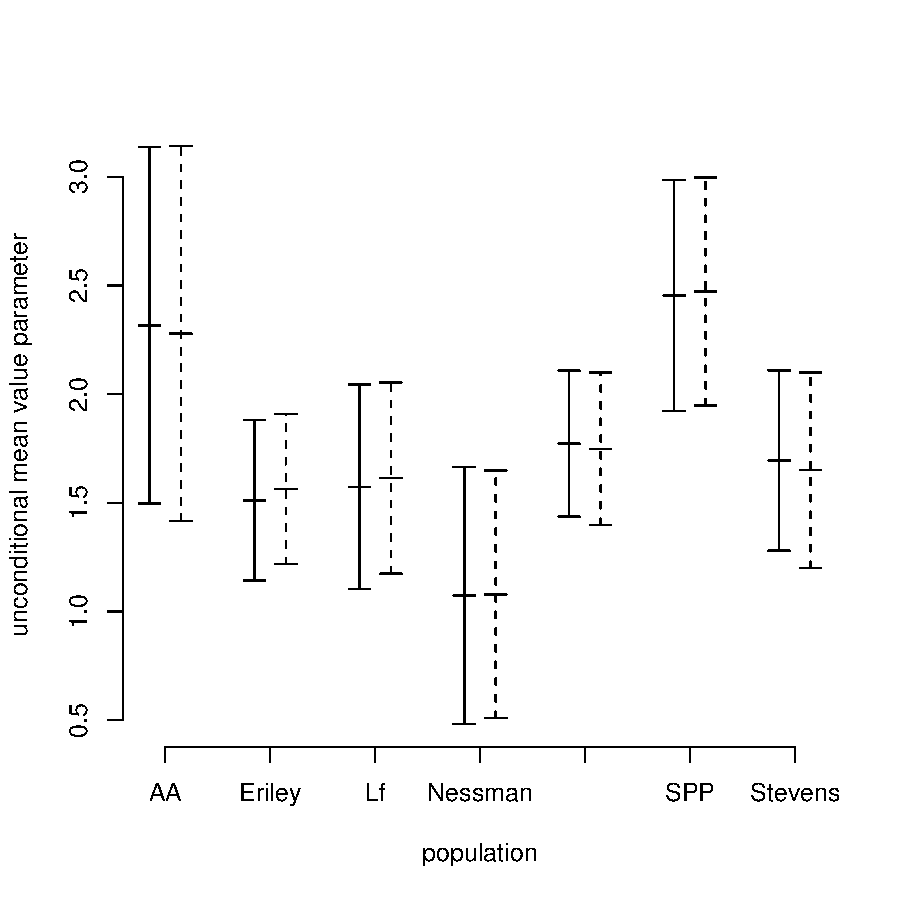
\includegraphics{tutor-fig1}
\end{center}
\caption{95\% confidence intervals for unconditional
mean value parameter for fitness (sum of head count for all years) at each
site for a ``typical'' individual having position zero-zero and having
the parameterization of Model~4 (solid bar) or Model~3 (dashed bar).
Tick marks in the middle of the bars are the center (the MLE).}
\label{fig:one}
\end{figure}

Figure~\ref{fig:one} looks pretty much like the plot in the paper.
It's a little different because the spatial part of the model (involving
\verb@ewloc@ and \verb@nsloc@ is simpler).

These confidence intervals have real-world meaning.  The parameters predicted
are ``components of fitness'' (expected flower head count over the course
of the experiment) for ``typical'' individuals (``typical'' spatial location
smack dab in the middle because we centered the spatial coordinates to
have median zero) at each of the sites.  (BTW I have no idea why \verb@axis@
leaves off one of the site labels when there's plenty of room.  To get this
plot right for the paper I just edited the PostScript file and put in the
missing label by hand.  If you ask me, it's a bug.  But the \verb@axis@
maintainer would probably say it's a feature.)

As we have seen, you can ``predict'' any kind of parameter
($\boldbeta$, $\boldtheta$, $\boldvarphi$, $\boldxi$, or $\boldtau$)
for any model.  All of the examples so far have been unconditional
aster models (FEF).  But we could have done everything above if
we had originally fit conditional aster models (CEF).

\section{Conditional Aster Models} \label{sec:conditional}

We could now repeat everything above \emph{mutatis mutandis}.
The only thing that would change is an argument \verb@type = "conditional"@
to any call to the \verb@aster@ function.  Then everything else works
exactly the same (of course the actual numerical results are different,
but the other function calls to \verb@summary.aster@, \verb@anova.aster@,
or \verb@predict.aster@ are meaningful without change).

Let's look at one example.
\begin{Schunk}
\begin{Sinput}
> cout4 <- aster(resp ~ varb + nsloc + ewloc + site * 
+     hdct - site, pred, fam, varb, id, root, data = redata, 
+     type = "cond")
> pcout4 <- predict(cout4, varvar = varb, idvar = id, 
+     root = root, newdata = renewdata, se.fit = TRUE, 
+     amat = amat)
\end{Sinput}
\end{Schunk}
Note that these are exactly the same as the commands that made
\verb@pout4@ except for the extra argument \verb@type = "cond"@
in the \verb@aster@ function call.  Thus we have fit a conditional
aster model (CEF) but predicted exactly the same $\boldA' \boldtau$
as in \verb@pout4@.

Figure~\ref{fig:two} compares these two ``predictions'' and is produced by the
following code
\begin{Schunk}
\begin{Sinput}
> sitenames <- as.character(newdata$site)
> fit3 <- pcout4$fit
> fit4 <- pout4$fit
> i <- seq(along = sitenames)
> foo <- 0.1
> y4top <- fit4 + crit * pout4$se.fit
> y4bot <- fit4 - crit * pout4$se.fit
> y3top <- fit3 + crit * pcout4$se.fit
> y3bot <- fit3 - crit * pcout4$se.fit
> plot(c(i - 1.5 * foo, i - 1.5 * foo, i + 1.5 * foo, 
+     i + 1.5 * foo), c(y4top, y4bot, y3top, y3bot), 
+     type = "n", axes = FALSE, xlab = "", ylab = "")
> segments(i - 1.5 * foo, y4bot, i - 1.5 * foo, y4top)
> segments(i - 2.5 * foo, y4bot, i - 0.5 * foo, y4bot)
> segments(i - 2.5 * foo, y4top, i - 0.5 * foo, y4top)
> segments(i - 2.5 * foo, fit4, i - 0.5 * foo, fit4)
> segments(i + 1.5 * foo, y3bot, i + 1.5 * foo, y3top, 
+     lty = 2)
> segments(i + 2.5 * foo, y3bot, i + 0.5 * foo, y3bot)
> segments(i + 2.5 * foo, y3top, i + 0.5 * foo, y3top)
> segments(i + 2.5 * foo, fit3, i + 0.5 * foo, fit3)
> axis(side = 2)
\end{Sinput}
\begin{Soutput}
NULL
\end{Soutput}
\begin{Sinput}
> title(ylab = "unconditional mean value parameter")
\end{Sinput}
\begin{Soutput}
NULL
\end{Soutput}
\begin{Sinput}
> axis(side = 1, at = i, labels = sitenames)
\end{Sinput}
\begin{Soutput}
NULL
\end{Soutput}
\begin{Sinput}
> title(xlab = "site")
\end{Sinput}
\begin{Soutput}
NULL
\end{Soutput}
\end{Schunk}
and appears on p.~\pageref{fig:two}.
\begin{figure}
\begin{center}
\begin{Schunk}
\begin{Soutput}
NULL
\end{Soutput}
\begin{Soutput}
NULL
\end{Soutput}
\begin{Soutput}
NULL
\end{Soutput}
\begin{Soutput}
NULL
\end{Soutput}
\end{Schunk}
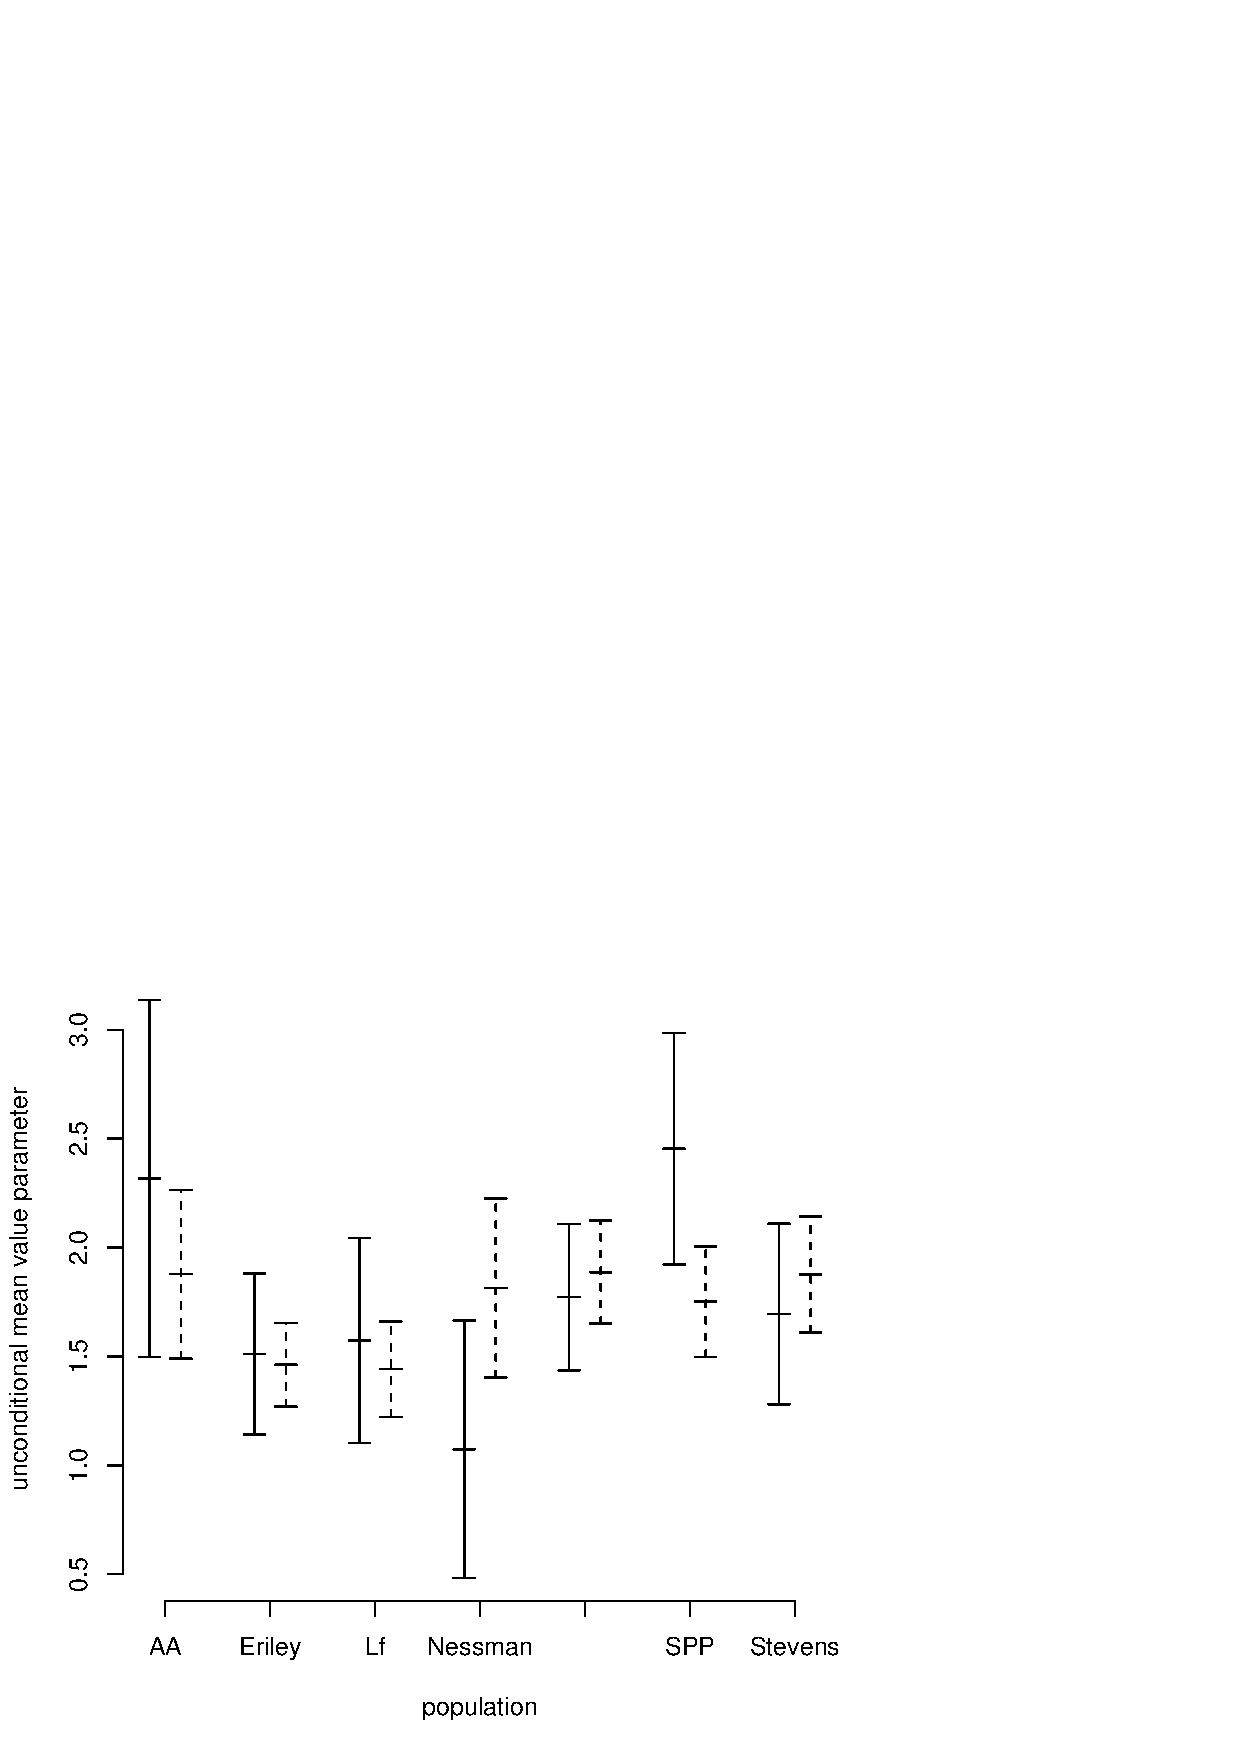
\includegraphics{tutor-fig2}
\end{center}
\caption{95\% confidence intervals for unconditional
mean value parameter for fitness (sum of head count for all years) at each
site for a ``typical'' individual having position zero-zero and having
the parameterization of Model~4, either an unconditional model (solid bar)
or conditional model (dashed bar).
Tick marks in the middle of the bars are the center (the MLE).}
\label{fig:two}
\end{figure}

Now note that the two types of intervals (solid and dashed) are wildly
different.  Of course, they \emph{should} be wildy different because
the two types of models, one with $\boldvarphi = \boldM \boldbeta$
and the other with $\boldtheta = \boldM \boldbeta$,
are radically different.  There is no reason for the two types of predictions
(of exactly the same thing) based on two radically different models should
be similar.  And they aren't.  So we are only seeing what we should expect
to see, an this doesn't prove anything about anything (except for the
trivial fact that FEF and CEF aster models are different).

\paragraph{Comment} We haven't really done justice to conditional models.
Since this is a tutorial, we don't have to.  As we said (twice), everything
is the same except for \verb@type = "cond"@ in the appropriate place.

And this is not the place to explain why one would want to use a conditional
or unconditional model.  And, to be honest, we don't know.  We know, and
explain in the paper, what each one does and why
\begin{quote}
Conditional aster models are simple algebraically,
but complicated statistically.

Unconditional aster models are complicated algebraically,
but simple statistically.
\end{quote}

But we have to admit that these arguments from theoretical statistics
may cut no ice with scientists, even if understood.  It all depends
on what particular scientific questions one is trying to answer.
Thus we have written the \verb@aster@ package to be completely even-handed
(except for defaults) with respect to conditional and unconditional
(models or parameters).  Whatever can be done with one kind can be done
with the other.  So use whatever you think right.

\section{Simulation}

One function we haven't covered is \verb@raster@ which simulates aster
models.  Let's check the coverage of some of our
so-called 95\% confidence intervals.

We start with another use of \verb@predict@.  The \verb@raster@ function
wants $\boldtheta$ or, to be more precise, here we use $\boldthetahat$.
\begin{Schunk}
\begin{Sinput}
> theta.hat <- predict(aout4, model.type = "cond", 
+     parm.type = "canon")
> theta.hat <- matrix(theta.hat, nrow = nrow(aout4$x), 
+     ncol = ncol(aout4$x))
> fit.hat <- pout4$fit
> beta.hat <- aout4$coefficients
\end{Sinput}
\end{Schunk}
We also need root data, and it will be simpler if we actually don't
use the forms of the \verb@aster@ and \verb@predict.aster@ functions
that take formulas
(because then we don't have to cram the simulated data in a data frame
and we avoid a lot of repetitive parsing of the same formulas)
\begin{Schunk}
\begin{Sinput}
> root <- aout4$root
> modmat <- aout4$modmat
> modmat.pred <- pout4$modmat
> x.pred <- matrix(1, nrow = dim(modmat.pred)[1], ncol = dim(modmat.pred)[2])
> root.pred <- x.pred
\end{Sinput}
\end{Schunk}
Now we're ready for a simulation
\begin{Schunk}
\begin{Sinput}
> set.seed(42)
> nboot <- 100
> cover <- matrix(0, nboot, length(fit.hat))
> for (iboot in 1:nboot) {
+     xstar <- raster(theta.hat, pred, fam, root)
+     aout4star <- aster(xstar, root, pred, fam, modmat, 
+         beta.hat, check.analyticals = FALSE)
+     pout4star <- predict(aout4star, x.pred, root.pred, 
+         modmat.pred, amat, se.fit = TRUE)
+     upper <- pout4star$fit + crit * pout4star$se.fit
+     lower <- pout4star$fit - crit * pout4star$se.fit
+     cover[iboot, ] <- as.numeric(lower <= fit.hat & 
+         fit.hat <= upper)
+ }
> pboot <- apply(cover, 2, mean)
> pboot.se <- sqrt(pboot * (1 - pboot)/nboot)
> cbind(pboot, pboot.se)
\end{Sinput}
\begin{Soutput}
     pboot   pboot.se
[1,]  0.91 0.02861818
[2,]  0.98 0.01400000
[3,]  0.94 0.02374868
[4,]  0.94 0.02374868
[5,]  0.91 0.02861818
[6,]  0.96 0.01959592
[7,]  0.94 0.02374868
\end{Soutput}
\end{Schunk}

Not bad for the small \verb@nboot@.  We won't try a serious simulation
because it would make this tutorial run too long.

\paragraph{Comment} The \verb@check.analyticals = FALSE@ argument
is passed to \verb@nlm@ which actually does the optimization.  (The
code we wrote only calculates the log likelihood and its derivatives.)
Other optimization options (calling \verb@optim@ are available), but
we haven't done extensive testing to see which is better (Hmmmm.  Well
on this job, using \verb@method = "L-BFGS-B"@ takes about four times
longer than the default and \verb@method = "CG"@ takes about eight times
longer.  So whatever problems \verb@optim@ is good for, it doesn't appear
to be strictly convex objective functions like aster models have.)
The starting parameter value \verb@beta.hat@ is supposed to speed things
up, giving the optimization a good starting point (the simulation truth),
but \verb@nlm@ still takes 150 iterations or so (not shown).

\end{document}

\begin{center} \LARGE REVISED DOWN TO HERE \end{center}

